\section{Das Environment}

Als Environment für die folgenden Experimente wollen wir eine Gebirgslandschaft erzeugen. Die Umgebung bildet hierbei ein Raster, worauf sich der Agent bewegen kann. Jeder Punkt auf dem Raster soll eine Höhe besitzen. Die Landschaft soll zufällig generiert werden können.

Die simpelste Lösung hierfür wäre wohl, ein zweidimensionales Array mit zufälligen Zahlen zu füllen. Auf diese Weise erhält man für jede Koordinate eine zufällige Höhe. Es ist allerdings für die Lesbarkeit des Problems essenziell, dass benachbarte Punkte einen Zusammenhang haben (zum Beispiel \glqq Bewegt sich der Agent gerade nach oben in die Richtung eines Gipfels oder nach unten in die Richtung eines Tals?\grqq). Dazu kommt, dass die Ergebnisse der Experimente intuitiv sichtbar sein sollen (zum Beispiel \glqq Hat der Agent einen Berg gefunden?\grqq). Deshalb wollen wir eine Landschaft erstellen, die organisch und natürlich aussieht.

% \subsection{Perlin Noise}
\paragraph{Perlin Noise}
Um dieses Ziel zu erreichen, verwenden wir \textit{Perlin Noise} \cite{parberry2015modeling}. Hierbei handelt es sich um eine Rauschfunktion, mit der sich sehr natürlich wirkende Texturen zufällig generieren lassen. Abbildung \ref{img:perlinNoise} zeigt eine simple Darstellung von zweidimensionalem Perlin Noise, bei der die generierten Werte mit Farbwerten von Schwarz bis Weiß abgebildet werden.
\begin{figure}[h!]
    \centering
    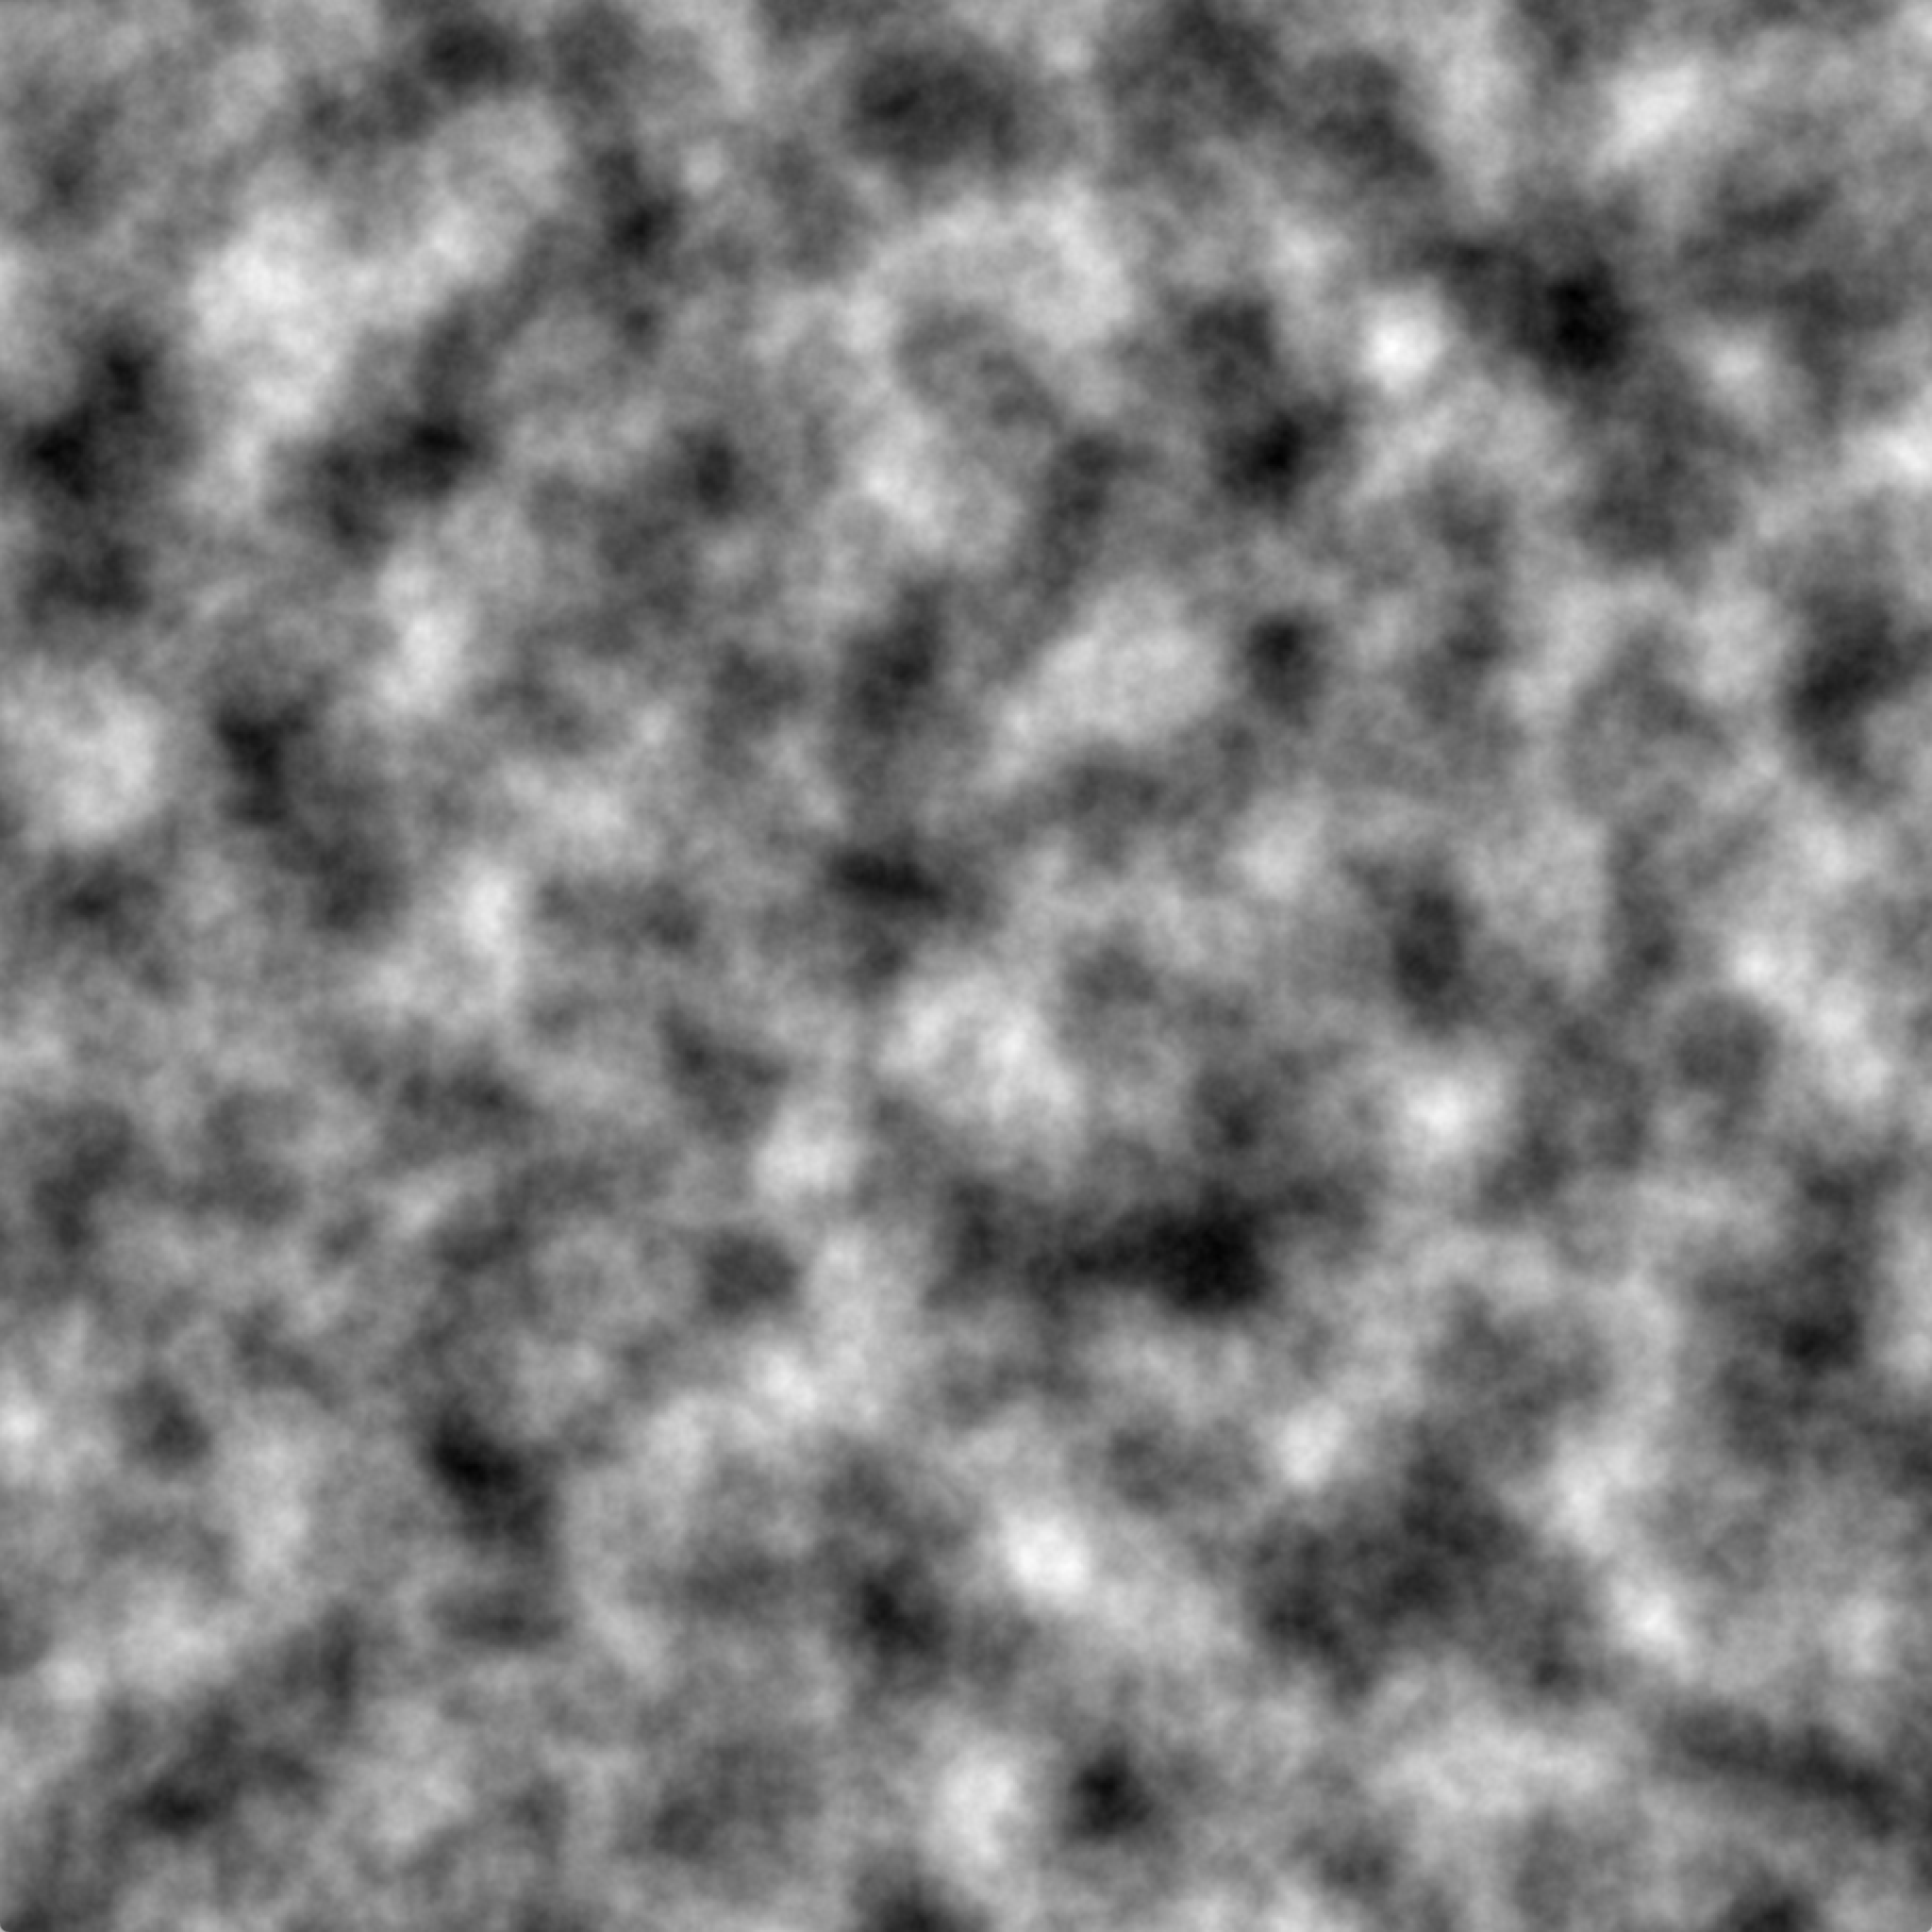
\includegraphics[width=0.5\textwidth, keepaspectratio=true]{perlin_noise.png}
    \caption{Visualisierung von zweidimensionalem Perlin Noise} \label{img:perlinNoise}
    \source{\url{https://miro.medium.com/max/2400/1*vs239SecVBaB4HvLsZ8O5Q.png}}
\end{figure}
Perlin Noise ist nach \cite{parberry2015modeling} ein fundamentaler Algorithmus in der prozeduralen Generierung von Terrain und somit offenbar sehr gut geeignet, um unsere Umgebung zu erstellen. Wir verwenden ihn um ein zweidimensionales Array mit zufälligen Werten zwischen -1 und 1 zu erzeugen, welche wir mit einer beliebigen Höhe multiplizieren können. Je nachdem, wie stark man in die Rauschfunktion \glqq hereinzoomt\grqq{}, erhält man unterschiedliche Verteilungen der Landschaft, wie man in Abbildung \ref{img:randomTerrain} erkennen kann.
\begin{figure}[h!]
    \centering
    \begin{subfigure}[b]{0.49\textwidth}
        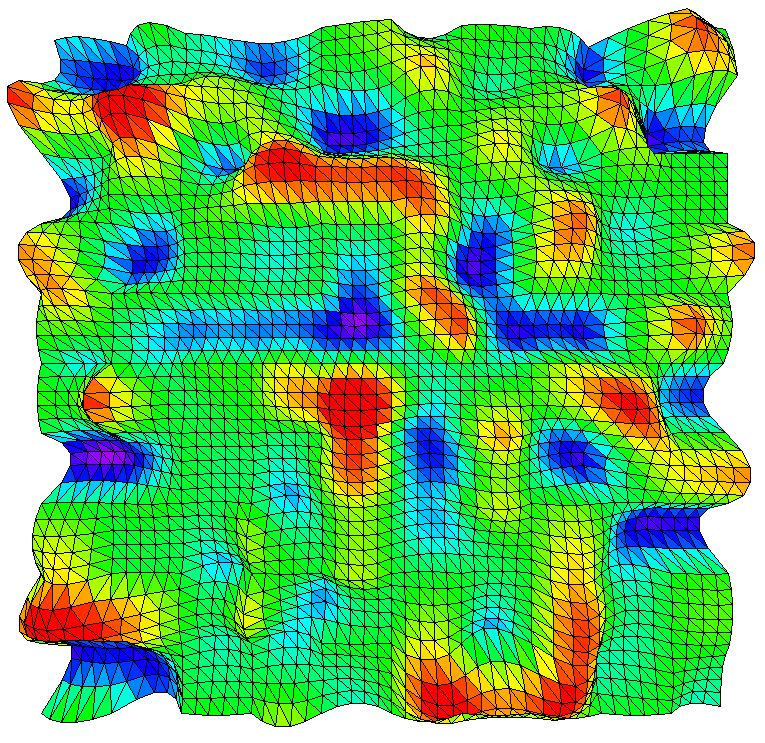
\includegraphics[width=\textwidth]{terrain_01.JPG}
        \caption{Landschaft mit niedriger Verteilung}
        \label{img:randomTerrainA}
    \end{subfigure}
    \begin{subfigure}[b]{0.49\textwidth}
        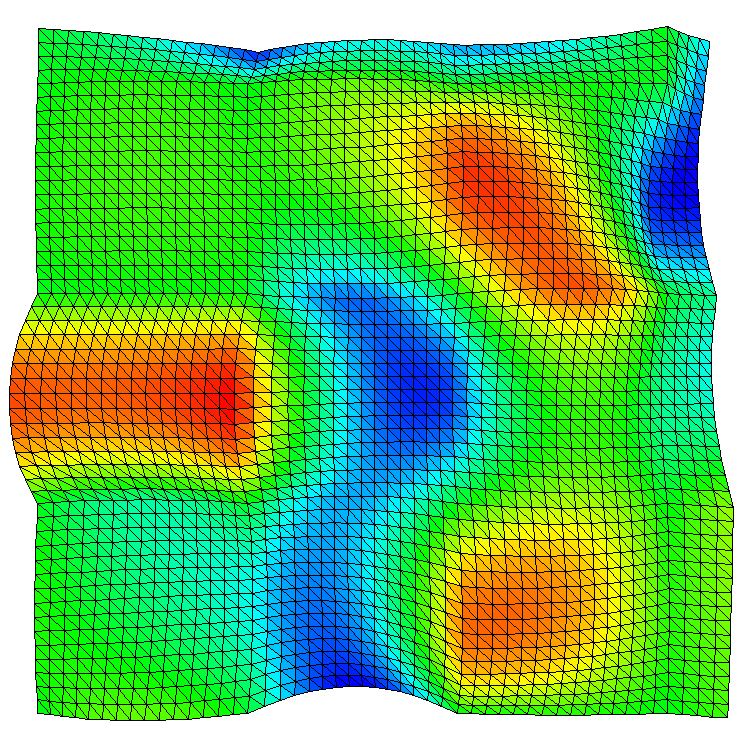
\includegraphics[width=\textwidth]{terrain_02.JPG}
        \caption{Landschaft mit hoher Verteilung}
        \label{img:randomTerrainB}
    \end{subfigure}
    \caption{Mittels Perlin Noise zufällig generierte Landschaften}
    \label{img:randomTerrain}
\end{figure}
Wir werden nicht näher auf die Details der Funktion eingehen, da dies nicht Kern dieser Arbeit ist. Für weitere Ausführungen diesbezüglich verweisen wir auf \cite{archer2011procedurally}.

Für die Visualisierung der Landschaft benutzen wir eine abgewandelte Form des Codes von \url{https://github.com/hnhaefliger/PyEngine3D} (Zugriff am 11.05.2021). Wir nutzen diese vergleichsweise simple 3D-Engine, damit wir alle Aspekte des Environments und dessen Visualisierung kontrollieren und für unseren Zweck anpassen können. So werden zum Beispiel zur besseren Differenzierung Berge und Täler -- zusätzlich zur perspektivischen Abhebung -- rot bzw. blau dargestellt.

Wir besitzen nun die Möglichkeit, eine zufällige Landschaft zu generieren und diese visuell darzustellen. Um bei allen Experimenten die gleichen Voraussetzungen zu gewährleisten, generieren wir mit der eben beschriebenen Methode zufällig ein Terrain, das allen folgenden Experimenten als Environment dient. Dieses ist in Abbildung \ref{img:terrainMain} dargestellt. Der höchste Punkt befindet sich bei dieser Landschaft auf dem Berg ganz oben in der Mitte.

\begin{figure}[h]
    \centering
    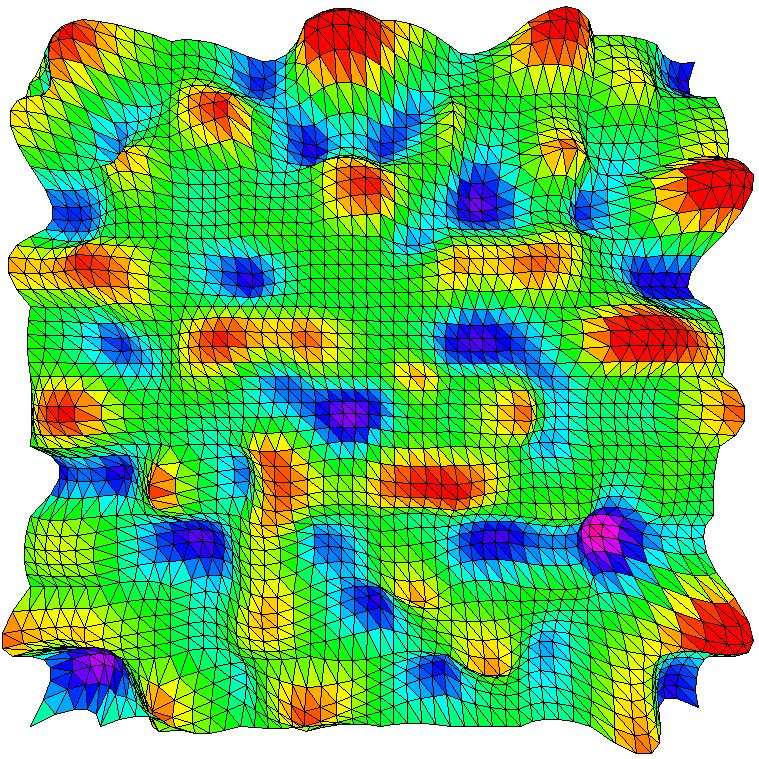
\includegraphics[width=0.5\textwidth, keepaspectratio=true]{terrain_main.JPG}
    \caption{Landschaft, auf der die Experimente durchgeführt werden} \label{img:terrainMain}
\end{figure}